\chapter{THE QUICK GUIDE TO THE VSM}\label{THE QUICK GUIDE TO THE VSM}
\noindent\fbox{
    \parbox{\textwidth}{%
        \centering
        \parbox{\textwidth - 6mm}{%%
            \vspace{3mm}
            In the following section, the entire VSM diagnosis is presented in brief.\\

            It will give you an overview of how the full diagnosis will proceed and of some of the diagrams which will be used.\\

            It will also enable those of you with some prior understanding and who have specific organisational problems to jump in at the sections that are most relevant.\\

            However, it should be stressed that until you have a reasonable understanding of the way in which the VSM looks at organisations, it may be difficult to grasp some of the concepts. If this proves to be the case, reading the Case Studies is perhaps the most accessible route to gaining the necessary background information.
            \vspace{3mm}
        }%%
    }%
}

\section*{Quick Guide: The Model}
The Viable Systems Model looks at an organisation interacting with its environment.

The organisation is viewed as two parts: \textbf{the Operation} which does all the basic work (production, distribution, earning the money) and the bits which provide a service to the Operation by ensuring the whole organisations works together in an integrated way (scheduling, accounts, strategic planning ...) These bits are called \textbf{the Metasystem}.

The following diagram illustrates the basic VSM.

\begin{longtable}[]{@{}
        >{\raggedright\arraybackslash}p{(\columnwidth - 2\tabcolsep) * \real{0.30}}
        >{\raggedright\arraybackslash}p{(\columnwidth - 2\tabcolsep) * \real{0.70}}@{}}
%    \endhead
    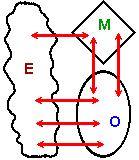
\includegraphics[width=\linewidth]{1vsm5}
    & \begin{minipage}[b]{\linewidth}\raggedright
        \begin{itemize}
            \item \textcolor{E}{\textbf{E}} represents the Environment
            \item \textcolor{O}{\textbf{O}} represents the Operation
            \item \textcolor{M}{\textbf{M}} represents the Metasystem
        \end{itemize}
    \vspace{\baselineskip}
    The arrows indicate the many and various ways that the three parts interact. Each arrow may have several aspects - it may be information, or trucks, a phone call or a delivery of steel ingots.
    \end{minipage} \\
\end{longtable}

The Operation will consist of a number of Operational units. These could be production units or teams of people doing various jobs.

The Metasystem can be divided in three main functions:

\begin{itemize}
  \item \textbf{The Internal Eye} - which looks at the entire collection of Operational units and deals with ways of getting them to work together in mutually beneficial ways, and with the resolution of conflicts. This is "Inside and Now".

  \item \textbf{The External Eye} - which looks at the external environment, assesses the threats and opportunities and makes plans to ensure the organisation can adapt to a changing environment. This is "Outside and Then".

  \item \textbf{Policy Systems} - which establish the ground rules which set the tone for the whole organisation. Policy rounds off the system. The policy systems must have ultimate control.

\end{itemize}

This is the basic model: The VSM sees any viable system as a collection of Operational elements which are held together by a Metasystem.

Both Operation and Metasystem must be in contact with, and interacting with, their environment.

The Operational units themselves must be viable, and thus can be looked at as smaller Viable Systems embedded in the larger system.

\section*{Quick Guide: The Model - Slightly Elaborated}

\begin{longtable}[]{@{}
        >{\raggedright\arraybackslash}p{(\columnwidth - 2\tabcolsep) * \real{0.60}}
        >{\raggedright\arraybackslash}p{(\columnwidth - 2\tabcolsep) * \real{0.40}}@{}}
    %    \endhead vsm-se5
    \raisebox{\normalbaselineskip-\height/2}{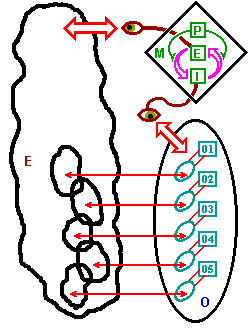
\includegraphics[width=\linewidth]{vsm-se5}}
    & \begin{minipage}[c]{\linewidth}\raggedright
       Note the three main parts - Operation, Environment and Metasystem.
       \vspace{\baselineskip}
       Note the Metasystem is shown with its internal and external eyes.
       \vspace{\baselineskip}
       Note the Operation is shown with five Operational units, all of which are smaller embedded Viable Systems
    \end{minipage} \\
\end{longtable}

\section*{Quick Guide: Preliminary Diagnosis}
In the Preliminary Diagnosis you look at your own organisation and examine the units which compose it. That is, you list the bits that do things, the co-ordination functions, the accounting and scheduling functions and so on.

You then draw a large VSM which will look something like the pictures on the previous pages to identify:

\begin{itemize}
  \item the Operational parts

  \item the parts which have inputs from the Internal Eye, and which deal with stability and optimisation of the Operational units.

  \item the parts which have inputs from the External Eye and which make long term plans in the light of Environmental information.

  \item the Policy Systems.

\end{itemize}

At the end of this process, you will have a large picture which gives a representation of your organisation in its totality.

This is the basic model from which the rest of the diagnosis will follow.

In some cases the Preliminary Diagnosis will be the most useful aspect. You may find that your organisation has no way to carry out some of the functions which are vital for viability. Thus, you may decide to create new jobs to ensure these functions get perfomed. You may also find that some jobs don't seem to have anything to do with the Viable Systems. You may decide they are not necessary.

\section*{Quick Guide: \hyperref[DESIGNING AUTONOMY]{Designing Autonomy}}
It is essential to create the right conditions for all the Operational units to function with as much autonomy as possible.

Thus they will need

\begin{itemize}
  \item Individual Mission Statements.

  \item Budgets for the resources they need to carry out this Mission.

  \item An agreement that they can decide on their own internal development as long as they are working to the agreed Mission.
\end{itemize}

There will also have to be safeguards to ensure that the units cannot threaten the overall viability of the organisation of which they are a part.

Thus

\begin{itemize}
  \item They must be accountable and able to demonstrate they are working to the agreed plan.

  \item There must be pre-agreed intervention rules which means that autonomy is forfeit under certain conditions. The worst case scenario must be considered in advance.

\end{itemize}

\section*{Quick Guide: Balancing the Internal Environment}
By this stage you will have looked at the various parts of you organisation and decided how they map onto the VSM. You will also have considered the autonomy of the Operational units.

The Internal Environment consists of all the Operational units and those jobs which are dedicated to looking at them (The Internal Eye) and to ensuring that conflicts are resolved and that their performance is optimised.

Internal balance is concerned with these (Metasystemic) jobs and with ensuring that they have the capabilities to function properly. So for example, a committee which meets once every three months would be an absurd idea - most of these jobs need to be done on a continuous basis.

The approach to Internal balance is as follows:

\begin{itemize}
  \item Maximise autonomy so that the vast majority of problems are dealt with within the Operational units.

  \item Examine the exchange of goods and services between the Operational units, and see if improvements may be made.

  \item Examine the bits of the external environment peculiar to each Operational unit and see if changes can be made (perhaps they all use the same suppliers and thus benefit from joint buying).

  \item Optimise the allocation of resources to the Operational units. It may be possible to cut back in one unit and re-invest in another, thus creating synergy in the whole system.

  \item Examine the scheduling and co-ordination functions.

  \item Ensure that the information systems which inform the Metasystem of the goings on at the Operational level are well designed. How complete is the information? How up-to-date is it?

  \item And lastly, after all the above have been exhausted, it may be necessary to "beef up" the capabilities of the Metasystem in order to ensure it can discharge its functions of overseeing the Operational units. This is the usual way that traditional businesses operate, and in terms of both efficiency and of human working conditions should be seen as the very last alternative.

\end{itemize}

The essence of the internal balance is to view the Inside of your enterprise as a system of autonomous Operational elements, which need to be overseen (the Internal Eye) to look for ways of generating synergy.

The imposition of dictates from \textit{above} should only be used when the viability of the whole enterprise is at risk and not, as in traditional businesses, as the usual way of dealing with most problems.

\section*{Quick Guide: Information Systems}
The VSM requires thorough and up-to-date information systems.

The perfect information system would measure everything it needs to know continuously, so that a real-time model of the goings on within any part of the enterprise may be maintained.

The compromise between this and the usual management information which is weeks or months out of date is the use of daily performance indicators.

These measure whatever is seen as important within each Operational units (productivity, morale, wastage, sales, breakages ...) at the end of each day. The figures are then plotted onto a time series so that the trends may be assessed.

\textbf{The essence of the VSM approach to information is that you only need to know if something changes.} If everything is going as normal, you can leave it alone. However as soon as something changes (dramatic fall in productivity) it's essential you are notified immediately.

Thus:

\begin{itemize}
  \item Huge printouts of standard information which say "\textit{nothing much has changed}" are useless.

  \item Immediate alerting signals which say "\textit{something dramatic has happened}" are essential.

\end{itemize}

These signals, which are called \textbf{algedonics}, are the basis of information handling in the VSM. They can be designed to provide Operational units with the information they need to learn and adapt to environmental changes, to define clear limits to autonomy, to guarantee that each Operational unit is working as an integrated part of the whole-system and so on.

The design of these information systems is crucial to the effective operation of your enterprise, and can be used as an alternative to authority.

\section*{Quick Guide: Balance with the Environment}
The External Eye maintains contact with the relevant parts of the external environment, and enables the future planning systems to develop strategies for adapting to change in the market, or to new technology, or whatever.

Again, the various parts must be balanced:

\begin{itemize}
  \item The future planning system must have the capabilities to examine and find the relevant information.

  \item It must be capable of planning and simulating various options.

  \item It must be aware of the capabilities of the Operational units, and develop any strategies within this context.

  \item It must be able to agree and implement its plans through the connections to the Operational units.

  \item It must function within policy guidelines.

\end{itemize}

\section*{Quick Guide: Policy Systems}
The policy systems oversee the entire organisation. They constitute the ultimate authority. Clearly they must be designed with great care.

For a co-operative it is crucial that everyone is involved in policy decisions and this usually involves a meeting of all members.

However, the practicalities of this need to be addressed. How often can the entire membership meet? How effective are big meetings? The answer to the question of how you involve all members in policy decisions and how you ensure that everyone has to work within these ground rules is perhaps one of the biggest questions for any Social Economy enterprise, and will determine the extent to which it may describe itself as democratic.

\section*{Quick Guide: Basic Vocabulary}
This Quick Guide to how the VSM looks at organisations and how it ensures the various parts are balanced has introduced most of the basic vocabulary.

\begin{itemize}
  \item Autonomous Operational units.

  \item Metasystem - concerned with ensuring the Operational units hang together or cohere into a single integrated organisation.

  \item Synergy - the added efficiency which comes from working together in a co-operative fashion.

  \item Daily Performance Indicators - which measure the goings on within each Operational unit.

  \item Algedonics - signals which are generated to say "Look out .. something unusual has occurred"

\end{itemize}

From now on, the manual will assume you understand these terms.

It will also use the five systems to describe the various functions within the organisation.

\begin{table}[H]
    \centering
\begin{tabular}{|C{0.14\textwidth} | L{0.79\textwidth}|}
    \hline
    \textbf{System 1} & The entire collection of interacting Operational units. \\
    \hline
    \textbf{System 2} & The system responsible for stability/resolving conflict between Operational units. \\
    \hline
    \textbf{System 3} & The systems responsible for optimisation/generating synergy between Operational units. \\
    \hline
    \textbf{System 4} & Future plans and strategies. Adaptation to a changing environment. \\
    \hline
    \textbf{System 5} & Policy. \\
    \hline
\end{tabular}
\end{table}